\chapter{Theory}


\section{PWFA - Linear-Fluid Wakefield Theory}
\subsection{Plasma Dynamics}
\textcolor{red}{What is the wave-breaking field $E_Z$, why is it the maximum possible acceleration/deceleration field? Is it always reached?}
\begin{equation}
\omega_p=\sqrt{\frac{4\pi e^2n_0}{me}}
\end{equation}
\subsection{Density perturbations}
Perturbation due to beam $n\left(r,\xi \right)\to n\left(r,\xi \right)+n_1\left(r,\xi \right)$, use Maxwell's equations and continuity equation.
\begin{equation}
-\frac{1}{k_p^2}\left(\frac{\partial^2 }{\partial \xi^2}+k_p^2\right)n_1\left(r,\xi \right)=n_b\left(r,\xi \right) ~,~~n_1\left(r,\xi<0 \right)=0
\end{equation}
\begin{equation}
\mathcal{L}_{\xi}n_1\left(r,\xi \right)=n_b\left(r,\xi \right) \quad \Rightarrow \quad \mathcal{L}_{\xi}G\left(\xi,\xi'\right)=\delta\left(\xi-\xi'\right)
\end{equation}
\begin{equation}
G\left(\xi,\xi'\right)=\left\{ \begin{array}{ll}
0 &,~ -\infty<\xi<\xi'\\
A\sin\left(k_p\xi \right) + B\cos\left(k_p\xi \right) &,~ \xi'<\xi<\infty
\end{array}\right.
\end{equation}
where the Green's function obeys the same b.c as the density perturbation, i.e it is continuous across the boundary with a discontinuous derivative across the boundary.
Integrate across discontinuity at $\xi=0$
\begin{equation}
\lim_{\epsilon\to 0}\int_{\xi'-\epsilon}^{\xi'+\epsilon} \mathcal{L}_{\xi}G\left(\xi,\xi'\right)\mathrm{d}\xi=\lim_{\epsilon\to 0}\int_{\xi'-\epsilon}^{\xi'+\epsilon}\delta\left(\xi\right)\mathrm{d}\xi=1 \quad \Rightarrow \quad \lim_{\epsilon\to 0}\left[-\frac{1}{k_p^2}\frac{\partial G}{\partial \xi}\right]^{\xi'+\epsilon}_{\xi'-\epsilon}=1
\end{equation}
Without loss of generality we may set the arrival of the beam to be at $t=0$, such that $\xi'=0$.
\begin{equation}
G\left(\xi,\xi'\right)=-k_p\sin\left(k_p\xi \right)\Theta\left(\xi \right) \quad \Rightarrow \quad n_1\left(r,\xi \right)=\int_{-\infty}^{\infty}G\left(\xi,\xi'\right)n_b\left(r,\xi' \right) \mathrm{d}\xi'
\end{equation}
\subsection{Longitudinal Accelerating Field} 
\begin{align}
&\boldsymbol{\nabla}\times \vec{E}=-\frac{1}{c}\frac{\partial \vec{B}}{\partial t} \\
&\boldsymbol{\nabla}\times \vec{B}=\frac{4\pi}{c}\vec{J}+\frac{1}{c}\frac{\partial \vec{B}}{\partial t}
\end{align}
gives
\begin{equation}
\nabla^2\vec{E}-\frac{1}{c^2}\frac{\partial^2 \vec{E}}{\partial t^2}=\frac{4\pi}{c^2}\frac{\partial \vec{J}}{\partial t}+4\pi\boldsymbol{\nabla}\rho
\end{equation}
Lorentz for law ($\vec{v}$ is the velocity of the plasma):
\begin{equation}
m\frac{\partial n\vec{v}}{\partial t}=en\left(\vec{E}+\frac{\vec{v}\times\vec{B}}{c} \right)\approx en\vec{E} \quad \Rightarrow \quad
\frac{\partial \vec{J}_p}{\partial t}=\frac{e^2 n}{m}\vec{E}
\end{equation}
Letting $\rho=\rho_b+\rho_p$ and $\vec{J}=\vec{J}_b+\vec{J}_p$ for the beam and plasma respectively, and $\vec{J}_b=c\rho_b\hat{\vec{z}}$, gives
\begin{equation}
\left(\nabla^2-\frac{1}{c^2}\frac{\partial^2}{\partial t^2}-k_p^2\right)\vec{E}=\frac{4\pi}{c}\frac{\partial \rho_b}{\partial t}\hat{\vec{z}}+4\pi\boldsymbol{\nabla}\left(\rho_b+\rho_p\right)
\end{equation}
where $k_p=\omega_p/c$ is the plasma wave number. To find the electric field along the beam, z-direction, we proceed by solving
\begin{equation}
\left(\nabla^2-\frac{1}{c^2}\frac{\partial^2}{\partial t^2}-k_p^2\right)E_z=\frac{4\pi}{c}\frac{\partial \rho_b}{\partial t}+4\pi\frac{\partial}{\partial z}\left(\rho_b+\rho_p\right)
\end{equation}
using $\nabla^2=\nabla^2_{\perp}+\partial^2_z$, in Fourier transform space, where\\
\textcolor{purple}{change this to E=integral tilde E, then substitute that into the following equations, since the RHS of 2.14 is not correct, fourier transform of the derivative acting on the function is not the same as the derivative acting on the transformed function}
\begin{equation}
E_z(\xi)\left(k\right)=\int_ {-\infty}^{\infty}\wtilde{E}_z(k)e^{ik\xi}\mathrm{d}k~~,~~~\left(\rho_b(k)+\rho_b(k)\right)=\int_ {-\infty}^{\infty}\left(\wtilde{\rho}_b\left(\xi\right)+\wtilde{\rho}_p\right)\left(\xi\right)e^{ik\xi}\mathrm{d}\xi
\end{equation}
such that 
\begin{equation}
\left(\frac{\partial^2 }{\partial z^2}-\frac{1}{c^2}\frac{\partial^2 }{\partial t^2}\right)E_z(\xi)=0
\end{equation}
and
\begin{equation}
\frac{4\pi}{c}\frac{\partial {\rho}_b}{\partial t}+4\pi\frac{\partial }{\partial z}\left({\rho}_b+{\rho}_p\right)=-4\pi i k\wtilde{\rho}_b+4i k\pi\wtilde{\rho}_b+4i k\pi\wtilde{\rho}_p=4i k\pi\wtilde{\rho}_p
\end{equation}
which gives 
\begin{equation}
\left(\nabla^2_{\perp}-k^2_p\right)\wtilde{E}_z\left(\xi\right)=4\pi i k\wtilde{\rho}_p
\end{equation}
We note that the two contributions from the beam cancel each other out, this is because of relativistic effects (?) \citep{Gessner2016}.
From eq. XXX we have
\begin{equation}
\frac{\partial^2{\rho}_p}{\partial t^2}+\omega_p^2{\rho}_p=-\omega_p^2{\rho}_b \quad \Rightarrow\quad
-k^2\wtilde{\rho}_p+k_p^2\wtilde{\rho}_p=-k_p^2\wtilde{\rho}_b \quad \Rightarrow\quad \wtilde{\rho}_p=\frac{k_p^2}{k^2-k_p^2}\wtilde{\rho}_b
\end{equation}

\begin{equation}
\nabla_{\perp}^2=\frac{1}{r}\frac{\partial }{\partial r}r\frac{\partial }{\partial r} +\frac{1}{r^2}\frac{\partial^2 }{\partial \phi^2} 
\end{equation}
\begin{equation}
 \left(\frac{\partial^2 }{\partial r^2}+\frac{1}{r}\frac{\partial }{\partial r} -k^2_p\right)\wtilde{E}_z
=4\pi ik_p^2 \frac{k}{k^2-k_p^2}\wtilde{\rho}_b
\label{diffeq_in_transformspace}
\end{equation}
We now rewrite this equation as
\begin{equation}
\mathscr{L}\wtilde{E}_z= \wtilde{f}(r)
\end{equation}
We proceed as before and solve this PDE by finding the Green's function. Working in a cylindrical coordinate system we have that the Green's function must satisfy 
\begin{equation}
\mathscr{L}G(\vec{r},\vec{r}')=\delta(\vec{r}-\vec{r}')=\frac{1}{r}\delta(r-r')\delta(\phi-\phi')\delta(z-z')
\end{equation}
where the RHS is the 3D Dirac delta function in cylindrical polar coordinates, defined such that 
$\int\delta(\vec{r}-\vec{r}')r\mathrm{d}r\mathrm{d}\phi\mathrm{d}z=1$. Letting 
\begin{equation}
G(\vec{r},\vec{r}')=G_r(r,r')\delta(\phi-\phi')\delta(z-z')
\end{equation}
leads to 
\begin{equation}
\mathscr{L}G_r(r,r')=\frac{1}{r}\delta(r-r')
\end{equation}
The LHS of this expression is the modified Bessel function of order zero and the RHS represents our source term. Consequently the Green's function is formed by linear combinations of, the linearly independent, modified Bessels functions of order zero. \todo{Standard Bessel function with complex arguments}
\begin{equation}
G\left(r,r'\right)=\left\{ \begin{array}{ll}
A(r')(A_1 I_0(k_pr)+B_1K_0(k_pr)) &,~ 0<r<r'\\
B(r')(A_2 I_0(k_pr)+B_2K_0(k_pr))  &,~ r'<r<\infty
\end{array}\right.
\end{equation}
requiring that the two parts of this expression each satisfy one of the B.Cs we have that $B_1=A_2=0$ since $K_0(k_pr)\to \infty$ as $r\to 0$ and $I_0(k_pr)\to \infty$ as $r\to \infty$. Continuity in $G(r,r')$ at $r=r'$ further gives that 
\begin{equation}
G\left(r,r'\right)=A_0\left\{ \begin{array}{ll}
I_0(k_pr)K_0(k_pr') &,~ 0<r<r'\\
I_0(k_pr')K_0(k_pr)  &,~ r'<r<\infty
\end{array}\right.
\end{equation}
where $A_0$ is a constant of proportionality that we find by integrating $\mathscr{L}G(r,r')=\delta(r-r')/r$ with respect to $r$ across the interval $\left[r'-\epsilon, r'+\epsilon \right]$, which needs to be satisfied for all $\epsilon$, including the limit as $\epsilon\to 0$.
\begin{align}
 \lim_{\epsilon\to 0}\int_{r'-\epsilon}^{r'+\epsilon}\left(\frac{\partial^2 G}{\partial r^2}+\frac{1}{r}\frac{\partial G}{\partial r} -k^2_pG\right)\mathrm{d}r= \lim_{\epsilon\to 0}\int_{r'-\epsilon}^{r'+\epsilon}\frac{1}{r}\delta(r-r')\mathrm{d}r&=\frac{1}{r'}\\
 \lim_{\epsilon\to 0}\Big[\frac{1}{k_p}\frac{\partial G}{\partial r} \Big]_{z-\epsilon}^{z+\epsilon}=\frac{A_0}{k_p} \left.\left(I_0(k_pr')\frac{\partial K_0(k_pr)}{\partial r}-\frac{\partial I_0(k_pr)}{\partial r}K_0(k_pr')\right)\right|_{r=r'} &=\frac{1}{r'}
\end{align}
\todo{find missing minus sign, check if a green's function can have r' in front, see judith's notes for what the constant of proportionality should be.}
This equality must hold for all values of $r'$. Hence, following an approach by Jackson \citep{Jackson1962}, we evaluate the LHS for $r'\gg 1$, where $I_0$ and $K_0$ take the limiting forms 
\begin{equation}
I_0(k_pr')\to \frac{1}{\sqrt{2\pi k_pr'}}e^{k_pr'} \quad \text{and} \quad K_0(k_pr')\to \sqrt{\frac{\pi}{2k_pr'}}e^{-k_pr'}
\end{equation}
which implies that $A_0=-1$. \textcolor{purple}{Here Gessner gets $A=4\pi$ because of Jackson but I don't see why.} 
\begin{equation}
G\left(r,r'\right)=- I_0(k_pr)K_0(k_pr')\Theta(r'-r)-I_0(k_pr')K_0(k_pr)\Theta(r-r')
\end{equation}
We can thus find $\wtilde{E}_z$ from 
\begin{equation}
\wtilde{E}_z(r,k)=\int_{-\infty}^{\infty}G\left(r,r'\right)f(r',k)r'\mathrm{d}r'
\end{equation}
and then perform an inverse Fourier transform to find 
\begin{equation}
E_z(r,\xi)=\frac{1}{2\pi}\int_ {-\infty}^{\infty}\wtilde{E}_z\left(r,k\right)e^{ik\xi}\mathrm{d}\xi
\end{equation}
Doing this yields 
\begin{align}
E_z(r,\xi)&=\frac{4\pi ik_p^2}{2\pi}\int_{-\infty}^{\infty}\frac{ke^{ik\xi}}{k^2-k_p^2}\mathrm{d}k\int_0^{\infty}G\left(r,r'\right)\wtilde{\rho}_b(r')r'\mathrm{d}r'\\
&=-2\pi k_p^2\cos(k_p\xi)\Theta(\xi)\int_0^{\infty}G\left(r,r'\right)\wtilde{\rho}_b(r')r'\mathrm{d}r'
\end{align}
Where the $\Theta(\xi)$ has been added due to causality.\\
Now lets solve this for a bi-Gaussian beam charge distribution. To do this, we may compute the electric field from the Green's function directly and then carrying out the inverse Fourier transform, or we could choose to first compute the field due to a point-particle and then convolving it with the bi-Gaussian distribution. We proceed by doing the latter by choosing a charge distribution with radial symmetry and a delta function in the $z$-direction to match our Green's function.
\begin{align}
{\rho}_{b_0}(r,\xi)=\frac{e}{2\pi r}\delta(r-r_0)\delta(\xi) \quad \Rightarrow\quad  \wtilde{\rho}_{b_0}(r,k)=\int_ {-\infty}^{\infty}\rho_b(r,\xi)e^{-ik\xi}\mathrm{d}\xi=\frac{e}{2\pi r}\delta(r-r_0)
\end{align}
which gives 
\begin{equation}
\wtilde{E}_z(r,k)=-2eik_p^2\frac{k}{k^2-k_p2}G\left(r,r_0\right)
\end{equation}
which satisfies (\ref{diffeq_in_transformspace}), as can be shown by integrating across the discontinuity and taking the limit to zero, and then gives
\begin{equation}
E_z(r,\xi)=-ek_p^2\cos(k_p\xi)G\left(r,r_0\right)\Theta(\xi)
\end{equation}
\textcolor{red}{But my Green's function has a $A=-1$ as constant and not $A=4\pi$ as Bonatto and Gessner}\\
This is refer to as the single-particle wake function \citep{Gessner2016}. The longitudinal electric field resulting from an arbitrary source distribution $n_b(r,\xi)$ is given by the convolution of the source by the single-particle wake function:
\begin{align}
E_z(r,\xi)&=-ek_p^2 \int_{-\infty}^{\infty} \cos(k_p(\xi-\xi'))\Theta(\xi-\xi')\mathrm{d}\xi' \int_{0}^{\infty}G\left(r,r_0\right) n_b(r_0,\xi')r'\mathrm{d}r'\\
&=-ek_p^2 \int_{-\infty}^{\xi} \cos(k_p(\xi-\xi'))\mathrm{d}\xi' \int_{0}^{\infty}G\left(r,r_0\right) n_b(r_0,\xi')r_0\mathrm{d}r_0
\end{align}
\textcolor{red}{which is not the same as Bonatto/Gessner/Schroeder, the limits are different, they have from xi to infity  , is this not how to do a convolution? Why don't we have somethign like $r-r'$ from a radial convolution or something? Bonatto, Schroder has the integral from infinity to xi, why? \\ These expressions with $-4\pi$ does not satisfy the diff.eq that I am trying to solve in transform space, so why do they use them if they don't solve their original diff. equations?\\ Mira's thesis also has $4\pi$ if converting to cgs.}
\subsection{Transverse Focusing Field} 



\clearpage
\section{Non-linear Regime} 
\subsection{Wave-breaking field}
\underline{Dawson's derivation}
We consider a simple 1D linear non-relativistic electron sheet model first used by Dawson \citep{Dawson1959} to show the breakdown of the linear model (\textcolor{red}{correct?}). Consider the plasma being made up of thin sheets of ions and electrons. A sheet at equilibrium position $z=z_0$ is then displaced by $\eta_0(z_0)$, where the displacement is set as function of the equilibrium position for full generality, to a new position $z=z_0+\eta_0$. The displaced sheet reveals a positive surface charge density $\sigma=en_0\eta_0$, where $n_0$ is the electron charge density in the plasma. This sets up a restoring electric field which we find using Gauss's law to be $E_{\text{res}}=4\pi n_0e\eta_0$ which yields a restoring force
\begin{equation}
 m_e\frac{\partial^2\eta_0}{\partial t^2}=-eE_{\text{res}}=-4\pi n_0e^2\eta_0=-\omega_p^2\eta_0
 \end{equation} 
 with solutions 
 \begin{equation}
 \eta_0(z_0,t)=A_1(z_0)\cos(\omega_p t)+A_2(z_0)\sin(\omega_p t)
 \end{equation}
The phenomena of wave breaking can be shown by considering another electron sheet at an equilibrium position $z_1=z_0+\Delta z_0$ at a distance $\Delta z_0$ away from the first sheet. This sheet is then displaced by $\eta_1$ to a new position $z^{*}_1=z_0+\Delta z_0+\eta_1$. The linear model is valid provided that there are no electron trajectories intersect one another in the plasma [ \textcolor{red}{is this correct? Why does the model break down?} ]. Hence the model is valid provided that $z^{*}_1-z_0>z-z_0$ which implies that we must have
\begin{equation}
\Delta z_0+\eta_1>\eta_0~,
\label{eta_ineq}
\end{equation}
for all $\Delta z_0\in \mathbb{R}$, to sustain plasma oscillations in the linear model. We now consider  the limit as $\Delta z_0\to 0$ for the expression 
\begin{equation}
\frac{\partial \eta}{\partial x_0}=\lim_{\Delta z_0\to 0}\frac{\Delta \eta}{\Delta z_0}=\lim_{\Delta z_0\to 0}\left(\frac{\eta_1-\eta_0}{\Delta z_0}\right)>\lim_{\Delta z_0\to 0}\left(\frac{\eta_0-\Delta z_0-\eta_0}{\Delta z_0}\right)=-1
\end{equation}
which simplifies to
\begin{equation}
\frac{\partial \eta}{\partial z_0}>-1
\label{no_crossing}
\end{equation}
where the inequality is introduced using Eq. (\ref{eta_ineq}). We now consider the special case where $A_1(z_0)=A\sin(k_pz_0)$ and $A_2(z_0)=0$. This is a valid solution since $\sin(k_pz_0)$ is single-valued for all $k_p,x_0\in\mathbb{R}$. This particular solution is chosen to highlight the breadown of the electric field, and is motivated by ([\textcolor{red}{what?}]) the solution we found for the electric field in section 2. Applying the no-crossing criterion in Eq. \ref{no_crossing} to $\eta=\eta_0(z_0,t)$ yields
\begin{equation}
\frac{\partial \eta_0}{\partial z_0}=Ak_p\cos(k_pz_0)>-1 \quad \Leftrightarrow \quad Ak_p\leq 1
\end{equation}
which gives the maximum amplitude as $A_{max}=1/k_p$. Hence the maximum restoring electric field $E_{max}\equiv E_{\text{wb}}=4\pi n_0/k_p$ is given by
\begin{equation}
E_{\text{wb}}=\frac{m_ev_p\omega_p}{e}
\end{equation}
the so-called \textit{wave-breaking field}. To further show how this breaks the linear model we consider the effect on the electric field up to and past the wave-breaking limit. As above we have, 
\begin{equation}
z=z_0+\eta_0=z_0+A\sin(k_p z_0)
\label{dawson_z}
\end{equation}
and 
\begin{equation}
E=4\pi n_0e A\sin(k_p z_0)
\label{dawson_E(z)}
\end{equation}
from which we want to find the electric field as a function of $z$. We can do this by numerically solving Eq. \ref{dawson_z} for $z_0$ in a range of $z$ values given fixed values of $A$. The gives $z_0=z_0(z,A)$ which can be substituted into Eq. \ref{dawson_E(z)} to give $E=E(z,A)$, the result of which is shown in Fig. \ref{DawsonCriterionPlot}. From this we conclude that the electric field is no longer single-valued for $A>1/k_p$, i.e past the electric field's wave-breaking amplitude, which signifies a breakdown of the linear model.\\
This is further emphasized by consider the electron-density response as $\partial \eta/\partial z_0\to -1$. To do this we use  Eq. XXX in 1D with no beam density $n_b=0$, 
\begin{equation}
\frac{\partial E}{\partial z}=4\pi e(n_0-n)
\end{equation}
where $n=n_0+n_1$ is the perturbed plasma density and $n_0$ is the ion density, hence $n_0-n$ is the free (negative) charge density in the plasma. We now take the derivative of the perturbed electric field and substitute the above expression
\begin{equation}
\frac{\partial E}{\partial z}=4\pi n_0 e \frac{\partial \eta}{\partial z} \quad \Rightarrow \quad n=n_0\left(1-\frac{\partial \eta}{\partial z}\right)
\end{equation}
We now rewrite $\partial /\partial z$, using $z=z_0+\eta$, as
\begin{equation}
\frac{\partial}{\partial z}=\left(1-\frac{\partial \eta }{\partial z_0}\right)^{-1}\frac{\partial}{\partial z_0}
\end{equation}
which gives
\begin{equation}
n=\frac{n_0}{1+\frac{\partial \eta }{\partial z_0}}
 \end{equation} 
 which means that the perturbed electron density grows infinite as $\partial \eta/\partial z_0\to -1$, again signifying the breakdown of the linear model.\\
\\
Having seen that the linear theory can break down mathematically, it is crucial to ask whether this is realised in 3D models and experiments as well. 
\begin{figure}
\centering
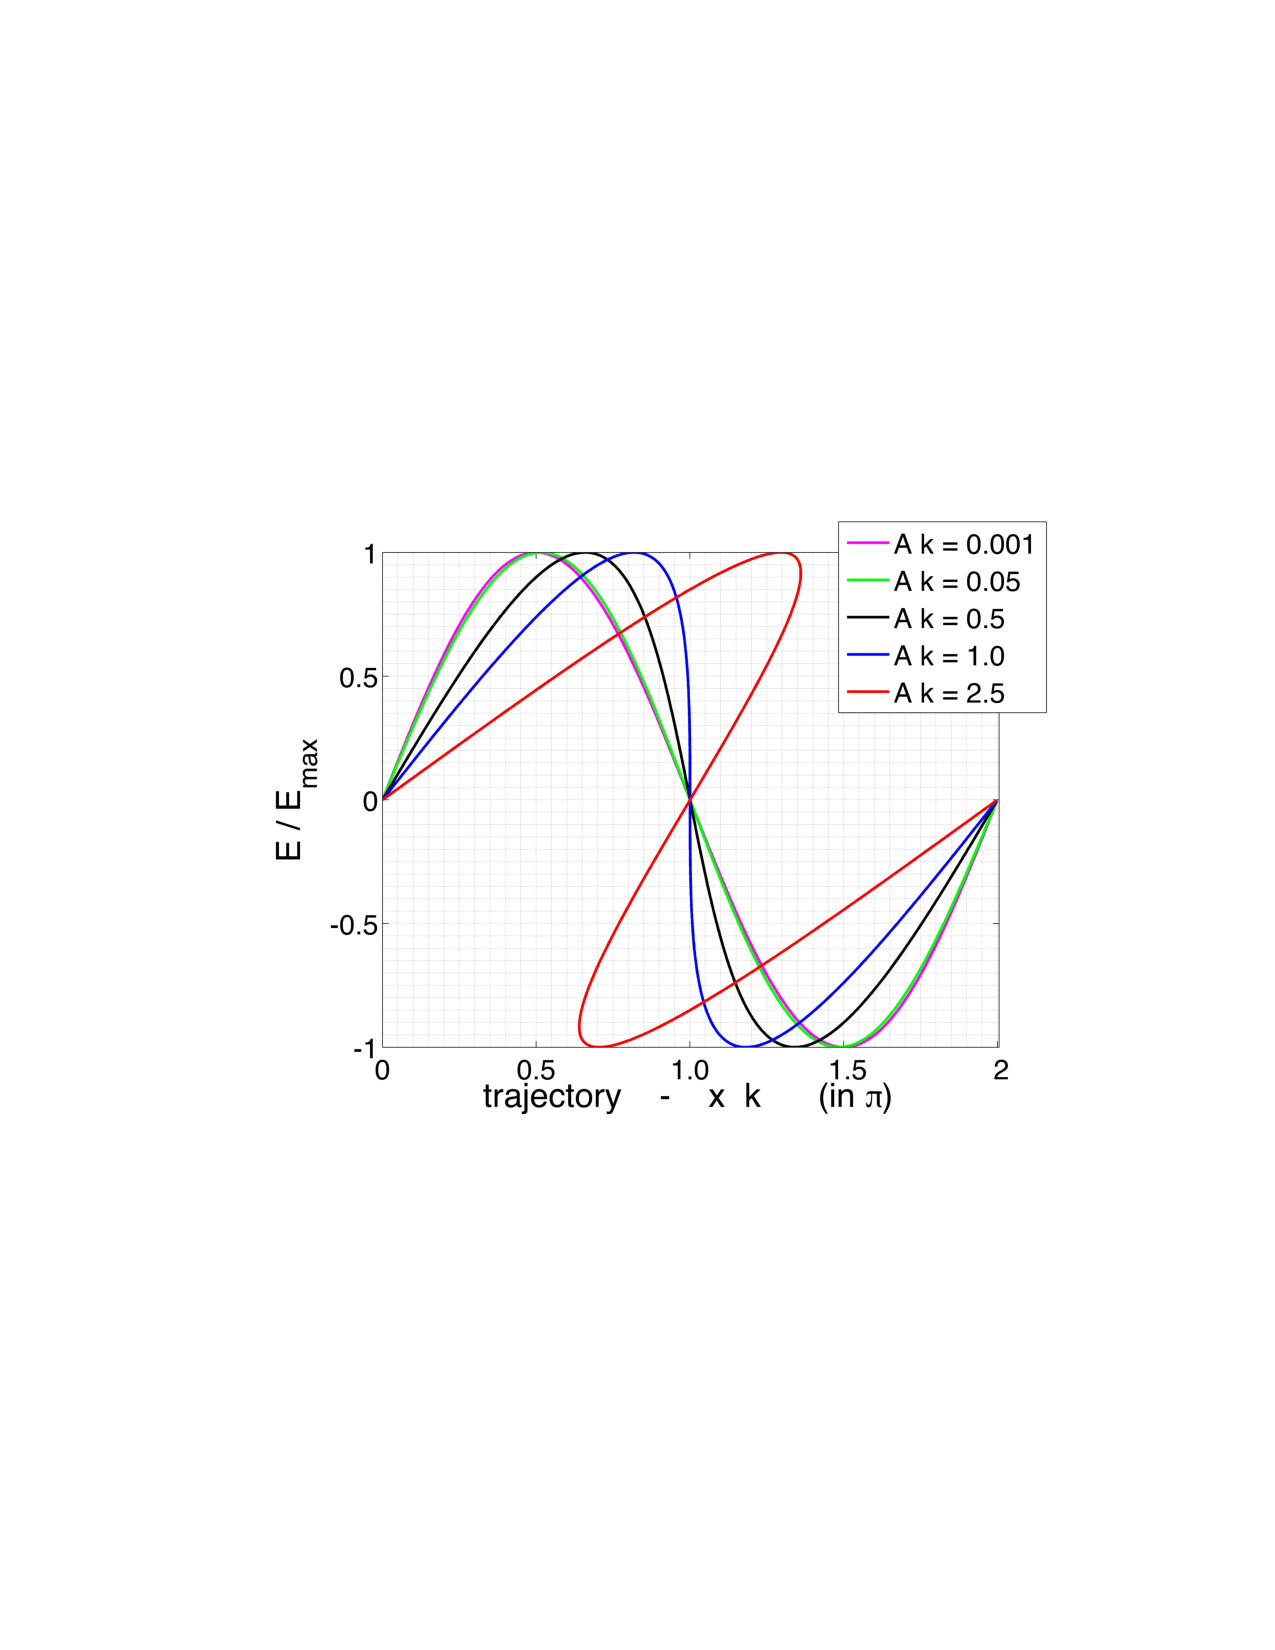
\includegraphics[scale=1]{SahaiThesisPlot}
\caption{Plot corresponding to Dawson's derivation of the wave-breaking field [ref. Sahai].}
\label{DawsonCriterionPlot}
\end{figure}

\clearpage
\section{Particle interactions with matter}
\subsection{Bohr-Fermi-Bethe-Bloch Theory}
Bethe-Bloch forumla:
\begin{equation}
-\expval{\frac{\mathrm{d}U}{\mathrm{d}s}}_{\text{ion}}=\frac{4\pi e^4n_{e,m}}{m_ec^2\beta^2}\left[\ln\left(\frac{2m_e\gamma^2v^2}{I}\right) -\beta^2\right]
\end{equation}

\subsection{Collective Plasma Deceleration}

\begin{equation}
-\left(\frac{\mathrm{d}E}{\mathrm{d}z}\right)_{\text{coll-wave-break}}=F_e=eE_{wave-break}=m_e c\omega_{p}\left(\frac{n_b}{n_e}\right)
\end{equation}

What is the wave-breaking electric field?

\subsection{Notes Bonatto}
Rate of change due to the longitudinal electric field acting on an electron beam, i.e position beam in the decelerating region of the wakefield.\\
"the beam only experiences its self-excited wakefield."\\
In the passive beam dump, are we essentially slowing down a "drive bunch" without having a witness bunch behind to get accelerated?\\
It is probaly better to use gamma as in Bonatto's paper, to make it easier to explain total beam energy integral. Basically integrate over all particles.\\
\\
$U=\gamma m_ec^2$
\begin{equation}
-\frac{\mathrm{d}U}{\mathrm{d}s}=(F_e)_z=eE_z
\end{equation}
where $s$ is the distance travelled in the plasma and $U$ is the energy of a particle in the beam at position $\xi$. 
for ultra relativistic beams, $\beta\sim 1$, the longitudinal electric field is a function of the position along the bunch $\xi=z-ct$ and not $z$ explicitly. 
\begin{equation}
U(s,\xi)=U_0-esE_z(\xi)
\end{equation}
The total energy of the beam after travelling a distance $s$ is then found by integrating across all the particles in the beam, which is integrating across $\xi$ since analysis is in 1-D.
\begin{equation}
\mathcal{U}(s)=U_0\int_{-\infty}
\end{equation}

